\documentclass[t,xcolor=pdftex,dvipsnames,table]{beamer}
\usepackage[]{graphicx}\usepackage[]{color}
%% maxwidth is the original width if it is less than linewidth
%% otherwise use linewidth (to make sure the graphics do not exceed the margin)
\makeatletter
\def\maxwidth{ %
  \ifdim\Gin@nat@width>\linewidth
    \linewidth
  \else
    \Gin@nat@width
  \fi
}
\makeatother

\definecolor{fgcolor}{rgb}{0.345, 0.345, 0.345}
\newcommand{\hlnum}[1]{\textcolor[rgb]{0.686,0.059,0.569}{#1}}%
\newcommand{\hlstr}[1]{\textcolor[rgb]{0.192,0.494,0.8}{#1}}%
\newcommand{\hlcom}[1]{\textcolor[rgb]{0.678,0.584,0.686}{\textit{#1}}}%
\newcommand{\hlopt}[1]{\textcolor[rgb]{0,0,0}{#1}}%
\newcommand{\hlstd}[1]{\textcolor[rgb]{0.345,0.345,0.345}{#1}}%
\newcommand{\hlkwa}[1]{\textcolor[rgb]{0.161,0.373,0.58}{\textbf{#1}}}%
\newcommand{\hlkwb}[1]{\textcolor[rgb]{0.69,0.353,0.396}{#1}}%
\newcommand{\hlkwc}[1]{\textcolor[rgb]{0.333,0.667,0.333}{#1}}%
\newcommand{\hlkwd}[1]{\textcolor[rgb]{0.737,0.353,0.396}{\textbf{#1}}}%
\let\hlipl\hlkwb

\usepackage{framed}
\makeatletter
\newenvironment{kframe}{%
 \def\at@end@of@kframe{}%
 \ifinner\ifhmode%
  \def\at@end@of@kframe{\end{minipage}}%
  \begin{minipage}{\columnwidth}%
 \fi\fi%
 \def\FrameCommand##1{\hskip\@totalleftmargin \hskip-\fboxsep
 \colorbox{shadecolor}{##1}\hskip-\fboxsep
     % There is no \\@totalrightmargin, so:
     \hskip-\linewidth \hskip-\@totalleftmargin \hskip\columnwidth}%
 \MakeFramed {\advance\hsize-\width
   \@totalleftmargin\z@ \linewidth\hsize
   \@setminipage}}%
 {\par\unskip\endMakeFramed%
 \at@end@of@kframe}
\makeatother

\definecolor{shadecolor}{rgb}{.97, .97, .97}
\definecolor{messagecolor}{rgb}{0, 0, 0}
\definecolor{warningcolor}{rgb}{1, 0, 1}
\definecolor{errorcolor}{rgb}{1, 0, 0}
\newenvironment{knitrout}{}{} % an empty environment to be redefined in TeX

\usepackage{alltt}
\newcommand{\SweaveOpts}[1]{}  % do not interfere with LaTeX
\newcommand{\SweaveInput}[1]{} % because they are not real TeX commands
\newcommand{\Sexpr}[1]{}       % will only be parsed by R


%\documentclass[handout,t,xcolor=pdftex,dvipsnames,table]{beamer}  % For handout
\mode<presentation>{
\useoutertheme[subsection=false]{miniframes}
%\beamertemplatenavigationsymbolsempty
\usecolortheme{custom}
\usefonttheme[onlymath]{serif}
\setbeamercovered{invisible}
%\setbeamertemplate{navigation symbols}{}
%\setbeamertemplate{mini frames}{}  % Old one
% Comment out this line to give the header
% \setbeamertemplate{headline}[default]
\setbeamertemplate{caption}[numbered]
%\setbeamertemplate{itemize items}[circle] 
\setbeamertemplate{frametitle continuation}{\frametitle{\color{white}Title}}  % So no tile on subsequent frames, from [allowframebreaks]

%%% CUSTOMISING NAVIATION %%%%
%This customises the navigation to be thin width and just have section headings (not subsections). 
\setbeamertemplate{headline}{%
\leavevmode%
  \hbox{%
    \begin{beamercolorbox}[wd=\paperwidth,ht=2.5ex,dp=1.125ex]{palette tertiary}%   % Tertiary colour is blue
    \insertsectionnavigationhorizontal{\paperwidth}{}{\hskip0pt plus1filll}
    \end{beamercolorbox}%
}}}

\RequirePackage{marvosym}

%%% INCLUDING SOLUTIONS %%%%
%% You can incorporate both questions and solutions in the 
%% same document.  Solutions can be included between the 
%% commands \begin{soln} and \end{soln}
%% To generate a pdf with only the questions uncomment:
%\excludecomment{soln}
\usepackage{comment}
\specialcomment{soln}{\begingroup \vspace{1mm} \sl}{ \leavevmode \endgroup}

%%%% DETAILS FOR PART 1 TITLE PAGE (OLD) %%%%
%\title{\large Part2 - Probability \& Distribution Theory} 
%\subtitle{} 
%\author{\copyright Dr Di Warren 2016} 
%\date{MATH1005 - Statistics}
% \colorlet{Faculty}{Arts}
%\colorlet{Faculty}{MasterBrandRed} % This is only needed if the notes are used for different faculties.
%\colorlet{FacultyText}{White}
% Defines the color of the text used on the title page and ``blocks''
% White for Business; TitlePageBlack for Arts, Pharmacy and Science
%\definecolor{CoolBlack}{rgb}{0.0, 0.18, 0.39}

%%%% DETAILS FOR FULL COURSE TITLE PAGE %%%%
\title{\Huge STATISTICS} 
\subtitle{} 
\author{\copyright University of Sydney 2017 (Di Warren)} 
\date{MATH1005}
% \colorlet{Faculty}{Arts}
\colorlet{Faculty}{MasterBrandRed} % This is only needed if the notes are used for different faculties.
\colorlet{FacultyText}{White}
% Defines the color of the text used on the title page and ``blocks''
% White for Business; TitlePageBlack for Arts, Pharmacy and Science
\definecolor{CoolBlack}{rgb}{0.0, 0.18, 0.39}

%%%% PACKAGES %%%%
\usepackage{multirow}
\usepackage{fancybox}
\usepackage[english]{babel}
\usepackage[utf8]{inputenc}
\usepackage{bm}
\usepackage{array}
\usepackage{booktabs}
\usepackage{tikz}
\usetikzlibrary{matrix,arrows,decorations.pathmorphing}
\usepackage{verbatim}
\usepackage{pgf,pgfsys,pgffor}
\usepackage{pgfplots}
\pgfplotsset{compat=1.3} %Recommended as of Pgfplots 1.3 - necessary?
\usetikzlibrary{decorations.pathreplacing,calc}
\usetikzlibrary{shapes, backgrounds}   % For Venn diagrams
\def \setA{ (0,0) circle (1cm) }
\def \setB{ (1.5,0) circle (1cm) }
\def \setC{ (0.6,1.5) circle (1cm) }
\def \setO{ (-2, -1.5) rectangle (3.5, 2.75) }
\tikzstyle{every picture}+=[remember picture]
\tikzstyle{na} = [baseline=-.5ex]
\usepackage{listings}  %Added by Di for adding R code

%\AtBeginSection[]
%{
%   \begin{frame}
 %      \frametitle{Outline}
 %      \tableofcontents[currentsection]
%   \end{frame}
%}  %This seems overkill for weekly lecture slides.

%\AtBeginSection[]
%{
%  \begin{frame}
% \frametitle{Contents}
%  \tiny{\tableofcontents[currentsection]}
%  \end{frame}
%}
%\useoutertheme{infolines} % Just lists current section in navigation at top, nice but limiting?

%%%% TITLE PAGE AND CONTENTS AT BEGINNING OF EACH TOPIC %%%%

\RequirePackage{ifthen} % package required
\newboolean{sectiontoc}
\setboolean{sectiontoc}{true} %default to true

\AtBeginSection[]
{
\begin{frame}[plain]
\vspace{60pt}
\begin{center}
\Huge{{\textcolor{MasterBrandBlue} \insertsection}}
\end{center}
\begin{tikzpicture}[scale=0.54]
%\hspace{-12pt}
%% Big Rectangle
\fill[MasterBrandRed] (0,14) -- (20,14) -- (20,15) -- (0,15);

%\draw (1,14.5) node [anchor = west] {\textcolor{MasterBrandBlue}{\Huge{\insertsection}}}; Overlays box with title, but long titles drop off the page
\end{tikzpicture} 
\end{frame}

%%%%%WORKING VERSION OF TOC%%%%%
%\begin{frame}
%   \frametitle{Outline}
%  \tableofcontents[currentsection, sectionstyle=show/hide, subsectionstyle=show/show/hide]
%  \end{frame}
%}

%%%%%2 VERSIONS - WITH AND WITHOUT TOC%%%%%
  \ifthenelse{\boolean{sectiontoc}}{
    \begin{frame}
  \frametitle{Outline}
  \tableofcontents[currentsection, sectionstyle=show/hide, subsectionstyle=show/show/hide]
 \end{frame}
  }
}
%%%%%This doesnt seem to work?%%%%
\newcommand{\toclesssection}[1]{
  \setboolean{sectiontoc}{false}
  %\section{#1}
  \setboolean{sectiontoc}{true}
}


% PDF settings
%\hypersetup{%
%  pdftitle={\inserttitle \insertsubtitle},%
%  pdfauthor={Di Warren},%
%	pdfsubject={},%
%	pdfkeywords={}%   
%	 }

%%%%  HELPFUL MACROS %%%%
\newcommand{\ud}{\mathrm{d}}
\newcommand{\var}{\mathrm{var}}
\newcommand{\ep}{\varepsilon}
\newcommand{\cov}{\mathrm{cov}}
\newcommand{\tr}{\mathrm{tr}}
\newcommand{\MSE}{\mathrm{MSE}}
\newcommand{\rank}{\mathrm{rank}}
\newcommand{\Bias}{\mathrm{Bias}}
\newcommand{\dei}{\partial}
\newcommand{\E}{\mathbb{E}}
\newcommand{\N}{\mathcal{N}}
\newcommand{\bbR}{\mathbb{R}}
\newcommand{\V}{\mathbb{V}}
\newcommand{\betahat}{\hat{\beta}}
\newcommand{\CLRM}{$\mathbf{y} = X\bm{\beta} + \bm{\ep}$}

%%%% LOGO FOR SLIDES %%%%
\logo{\vspace{79mm}
\includegraphics[height=0.9cm]{../images/sydney.pdf}}

%%%% ADD PAGE NUMBER %%%%
\setbeamertemplate{sidebar right}{}
\setbeamertemplate{footline}{%
\hfill\usebeamertemplate***{navigation symbols}
\hspace{1cm}\insertframenumber{}/\inserttotalframenumber}

%%%% BEGIN CONTENT %%%


\begin{document}



%%%% TOPIC9 %%%%
\section[9]{Topic9: Test for Proportion (Proportion and Sign Tests)}

\subsection[Example]{Example1: IVF}
\begin{frame}{Example1: IVF}

IVF (In Vitro Fertilisation) is a technique of assisted reproductive technology.
The first IVF baby was born in Australia in 1980 under the supervision of a team of doctors at Monash University, the 3rd IVF baby in the world. The first IVF baby was born in the UK (Louise Brown, 25 July 1978, physiologist and Nobel Prize Winner Sir Robert Edwards, surgeon Dr Patrick Steptoe).

\vspace{.5cm}
Interestingly, of the first 7 IVF births in Australia, 6 were girls. {\bf Is there evidence of a gender bias in IVF?}

\begin{center}
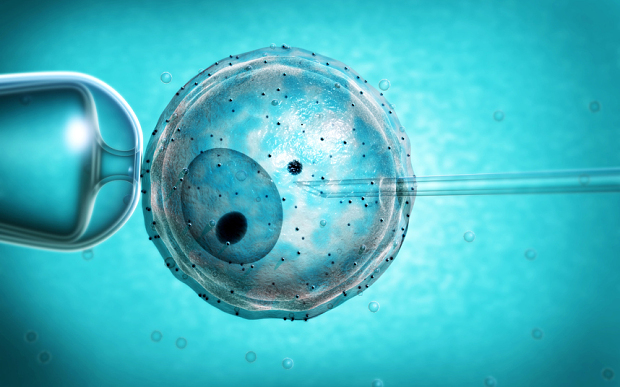
\includegraphics[height=3cm]{../images/IVF.jpg}
\end{center}
\end{frame}

\subsection[Example]{Example2: Vegetarianism in Australia}
\begin{frame}{Example2: Vegetarianism in Australia}
According to data from 2013, 10\% of the Australian population choose a vegetarian diet. In 2015, a survey of 10,000 people resulted in 1,190 vegetarians.
{\bf Has vegetarianism increased in Australia?}

\begin{center}
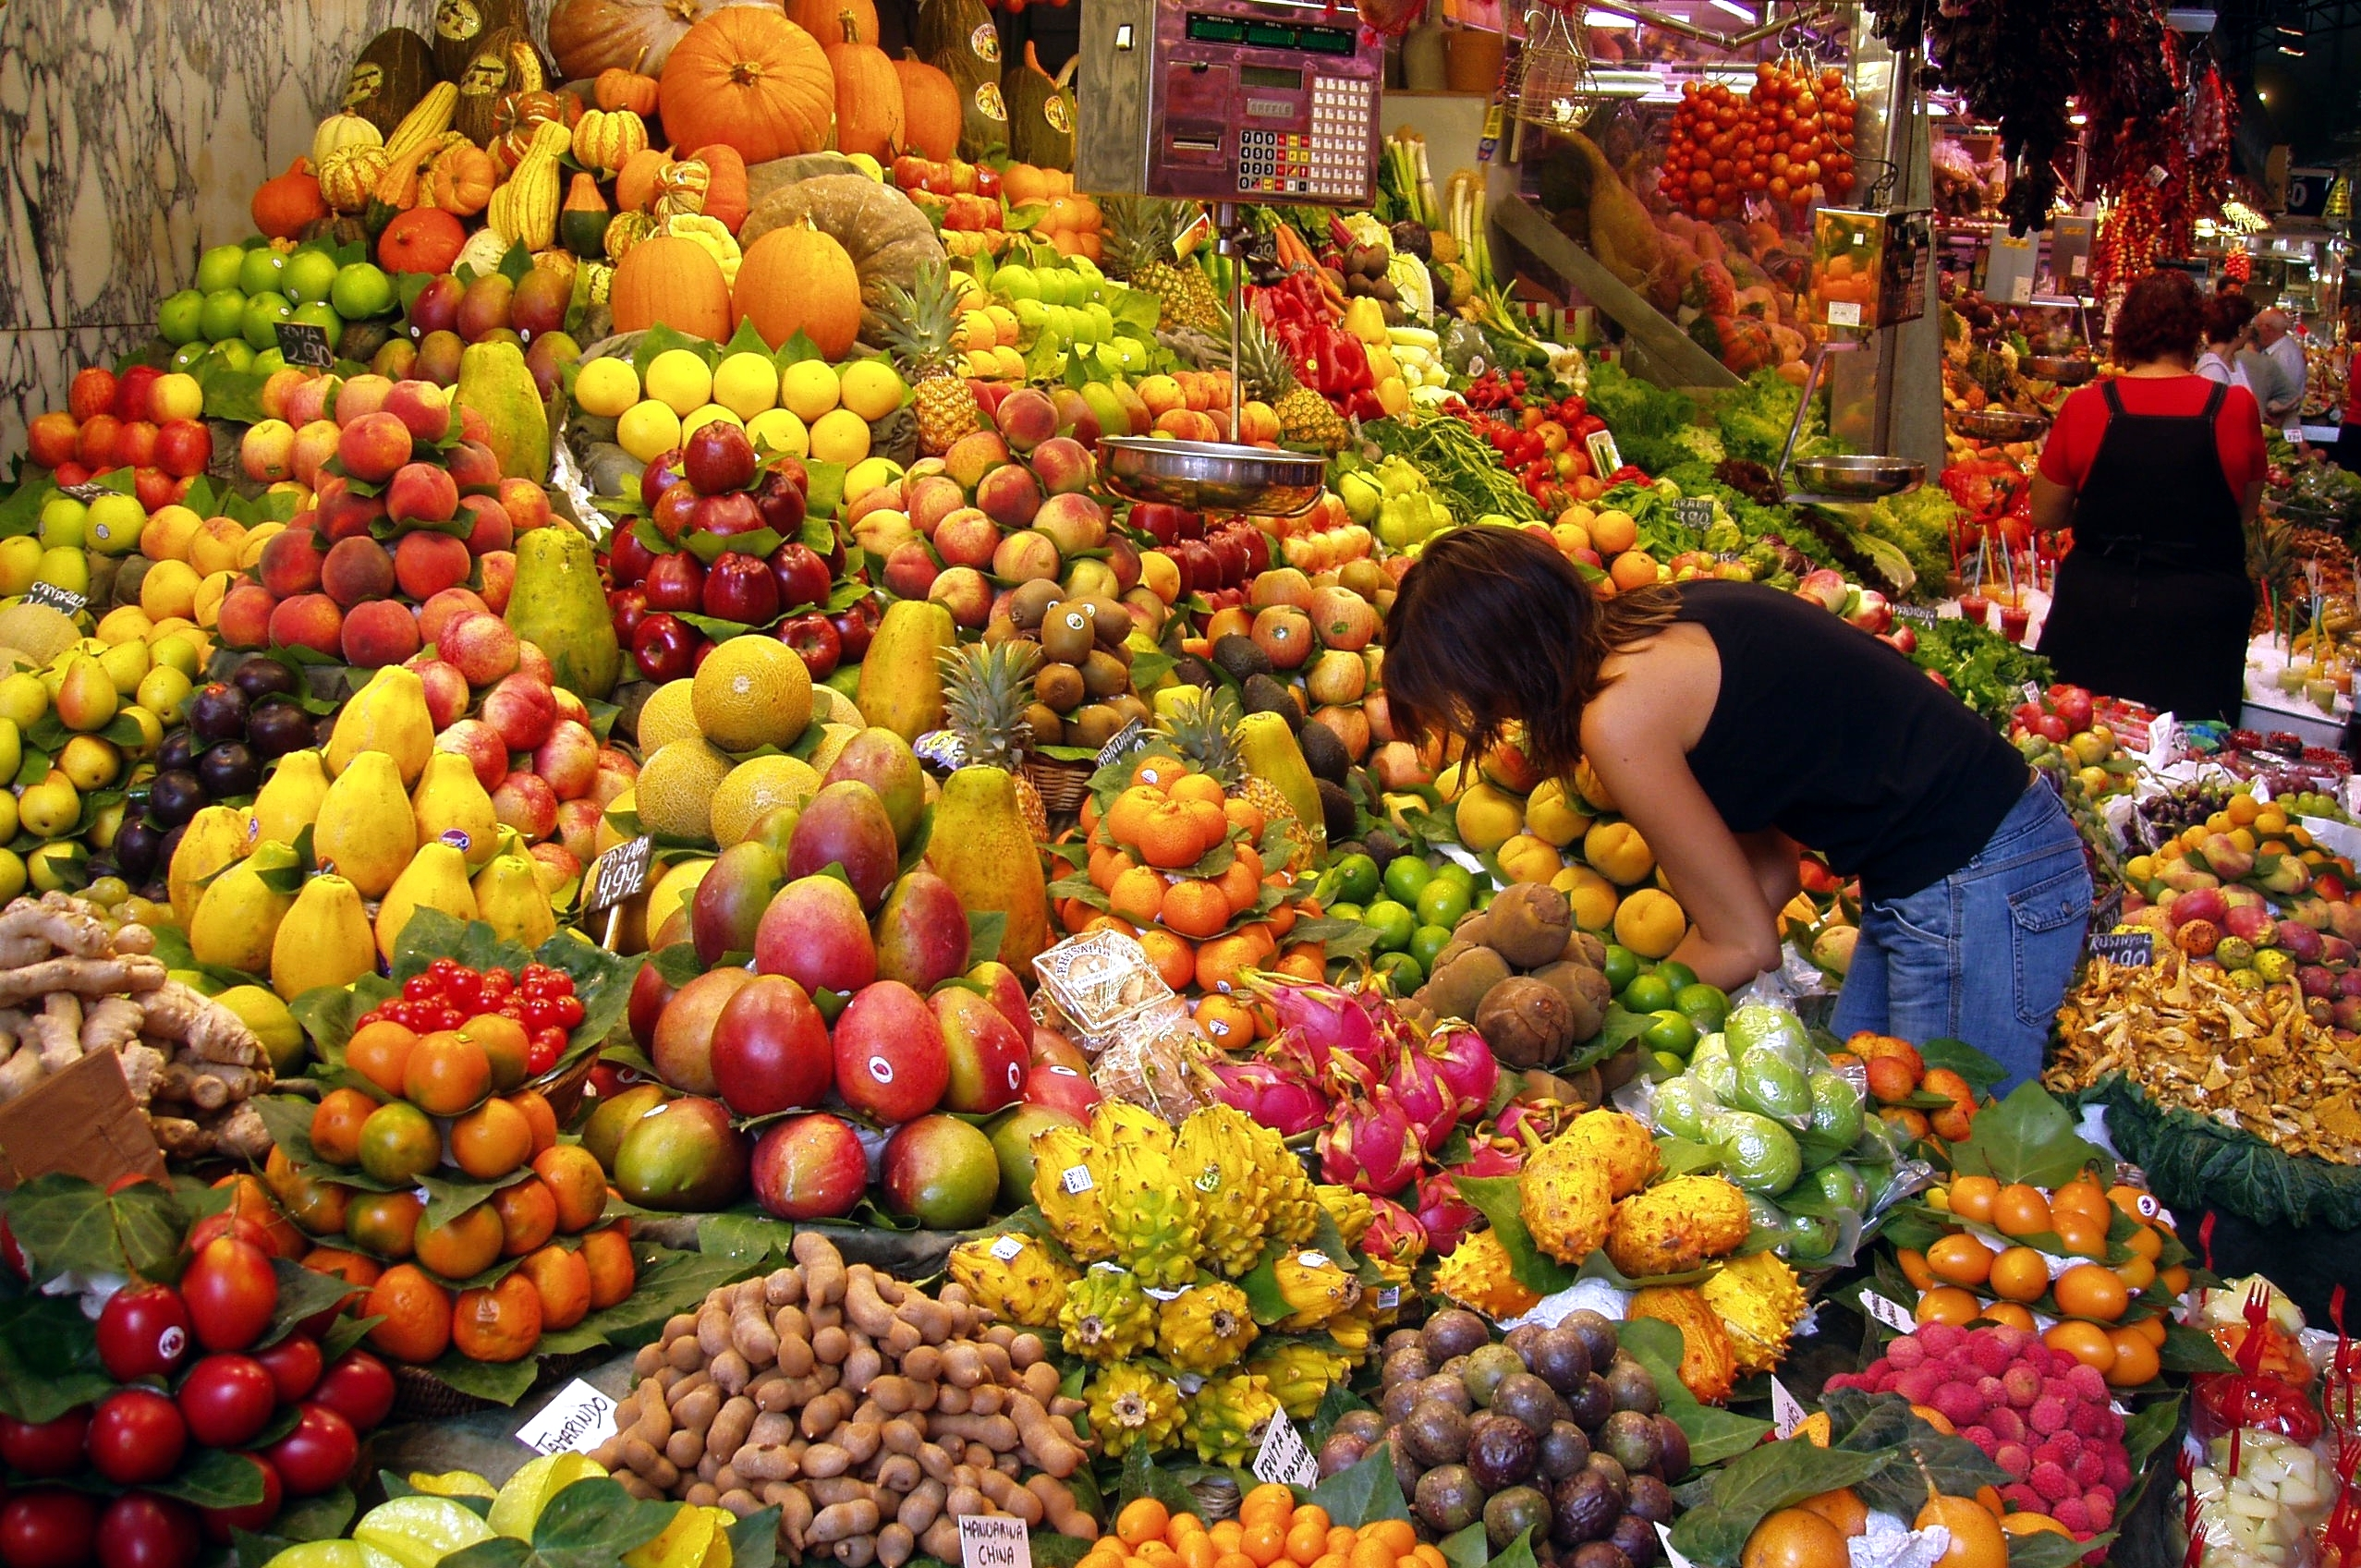
\includegraphics[height=4cm]{../images/BarcelonaFruit.jpg}
\end{center}
\href{http://www.roymorgan.com/findings/5264-meat-free-health-conscious-anxious-australias-vegetarians-201310272327}{\beamergotobutton{Roy Morgan Stats}}
\end{frame}

\subsection[Intuitive Approach]{An intuitive approach to the Proportion Test}
\begin{frame}{An Intuitive approach to the Proportion Test}

Select a coin from your wallet. {\bf Is the coin biased?}

\vspace{.5cm}
\framebox{Hypothesis} $H_{0}$: Coin is fair, $p=P(Head) = 0.5$. \\

\framebox{Experiment} Toss the coin 20 times and see how many heads come up. \\

\framebox{Observed Sample} This results in $x$ heads. \\

\framebox{Conclusion} If the number of heads $x$ is very small or very big, then there is evidence against $H_{0}$.
\end{frame}

\begin{frame}[fragile]{}

Assuming $H_{0}$ is true, then $X = \mbox{Number of heads} \sim Bin(n=20,p=0.5)$. \\

\vspace{.5cm}
\begin{tabular}{lll} \hline
$x$ & $P(X \mbox{is } x \mbox{ or more extreme})$ & Conclusion \\ \hline
0 & $P(X =0) =0.00000095$ & $H_{0}$ is highly unlikely. \\
1 & $P(X \leq 1) =0.00002$ & $H_{0}$ is highly unlikely. \\
2 & $P(X \leq 2) =0.0002$ & $H_{0}$ is highly unlikely. \\
5 & $P(X \leq 5) =0.02$ & $H_{0}$ is fairly unlikely. \\
8 & $P(X \leq 8) =0.25$ & Data consistent with $H_{0}$. \\ \hline
\end{tabular}

{\tiny 
\begin{knitrout}
\definecolor{shadecolor}{rgb}{0.969, 0.969, 0.969}\color{fgcolor}\begin{kframe}
\begin{alltt}
\hlstd{x}\hlkwb{=}\hlkwd{c}\hlstd{(}\hlnum{0}\hlstd{,}\hlnum{1}\hlstd{,}\hlnum{2}\hlstd{,}\hlnum{5}\hlstd{,}\hlnum{8}\hlstd{)}
\hlkwd{pbinom}\hlstd{(x,}\hlnum{20}\hlstd{,}\hlnum{0.5}\hlstd{)}
\end{alltt}
\begin{verbatim}
## [1] 9.536743e-07 2.002716e-05 2.012253e-04 2.069473e-02 2.517223e-01
\end{verbatim}
\end{kframe}
\end{knitrout}
}
\end{frame}


\subsection[Proportion]{Steps for Proportion Test}
\begin{frame}[fragile]{Steps for Proportion Test}
For a hypothesis concerning a unknown population proportion $p$, we follow the following steps. \\

\vspace{.5cm}
\framebox{H} $H_{0}: p = p_{0}$ vs $H_{1}: p < p_{0}$. \\

\framebox{A} The $n$ trials are independent with constant probability $p$.

\framebox{T} 
\begin{itemize}
\item $\tau = X =  \mbox{number of successes} \sim Bin(n,p_{0})$ under $H_{0}$. 
\item Small values of $x$ will argue against $H_{0}$ for $H_{1}$. 
\item The observed value is $x$. 
\end{itemize}

\framebox{P} $P$-value = $P( X \leq x)$.

\framebox{C} Weigh up the $P$-value. A rule of thumb is to reject $H_{0}$ for $P$-value $< 0.05 = \alpha$.
\end{frame}  

\begin{frame}{}
Notes on $P$-value:

\begin{itemize}
\item If the alternate hypotheses is $H_{1}: p > p_{0}$, then large values of $x$ will argue against $H_{0}$ for $H_{1}$ and the associated $P$-value is $P( X \geq x)$. 
\item If the alternate hypotheses is 2 sided $H_{1}: p \neq p_{0}$, then both small and large values of $x$ will argue against $H_{0}$ for $H_{1}$ and the associated $P$-value is $P( |X-n p_{0}| \geq |x-n p_{0}|)$.
\item In the special case when $p_{0} = \frac{1}{2}$, the 2 sided $P$-value reduces to
\begin{itemize}
\item $P$-value $= 2P( X \geq x)$, for $x > \frac{n}{2}$.
\item $P$-value $= 2P( X \leq x)$, for $x < \frac{n}{2}$.
\end{itemize}
\item If $n$ is large, then we can use the CLT (Topic 7) to find an approximation to the $P$-value. We find the approximating Normal $Y \sim N(n p_{0}, n p_{0} (1-p_{0}))$, and then either use R or standardise the Normal and look up the Normal tables.
\end{itemize}
\end{frame}

\begin{frame}{Examples}
\begin{block}{IVF}
Of the first 7 IVF births in Australia, 6 were girls. Is there evidence of a gender bias in IVF?
\end{block}

\vspace{.5cm}
Let $p = P(\mbox{girl baby from IVF)}$. Note this is a 2 sided test as the possible direction of bias is unspecified, given this was the first IVF trials.

\vspace{.5cm}
\framebox{H} 
Without prior evidence, we would assume no gender bias, hence $p_{0} = 0.5$. If there is a gender bias, then $p_{0} \neq 0.5$.  \\
Hence,  $H_{0}: p = 0.5$ vs $H_{1}: p \neq 0.5$. \\

\vspace{.5cm}
\framebox{A} The $n=7$ births are independent with constant probability $p$.

\end{frame}


\begin{frame}[fragile]{}

\framebox{T} 
\begin{itemize}
\item $\tau = X =  \mbox{number of girl births from 1st 7 IVF births} \sim Bin(7,0.5)$ under $H_{0}$. 
\item Small and large values of $x$ will argue against $H_{0}$ for $H_{1}$. \\
(ie if $H_{0}$ is not true, then we would expect $x$ to indicate either a bias towards girls (large) or bias towards boys (small)).
\item The observed value is $x=6$ (large).
\end{itemize}

\vspace{.5cm}
\framebox{P} $P$-value = 2 $P( X \geq 6)$ = 0.125.

\begin{knitrout}
\definecolor{shadecolor}{rgb}{0.969, 0.969, 0.969}\color{fgcolor}\begin{kframe}
\begin{alltt}
\hlkwd{dbinom}\hlstd{(}\hlnum{6}\hlstd{,}\hlnum{7}\hlstd{,}\hlnum{0.5}\hlstd{)} \hlopt{+} \hlkwd{dbinom}\hlstd{(}\hlnum{7}\hlstd{,}\hlnum{7}\hlstd{,}\hlnum{0.5}\hlstd{)}
\end{alltt}
\begin{verbatim}
## [1] 0.0625
\end{verbatim}
\begin{alltt}
\hlnum{1}\hlopt{-}\hlkwd{pbinom}\hlstd{(}\hlnum{5}\hlstd{,}\hlnum{7}\hlstd{,}\hlnum{0.5}\hlstd{)}
\end{alltt}
\begin{verbatim}
## [1] 0.0625
\end{verbatim}
\end{kframe}
\end{knitrout}
\end{frame}


\begin{frame}[fragile]{}

\framebox{C} 
As the $P$-value is 12.5\%, we would say that the data are consistent with $H_{0}$. Hence, it appears that there is not a gender bias in IVF.\\

\vspace{.5cm}
Note: What the $P$-value indicates, is that getting $x=6$ or greater ($x=7$) on a Binomial(7,0.5) distribution is not that uncommon, which is clear from the Binomial probability distribution function.

\begin{knitrout}
\definecolor{shadecolor}{rgb}{0.969, 0.969, 0.969}\color{fgcolor}
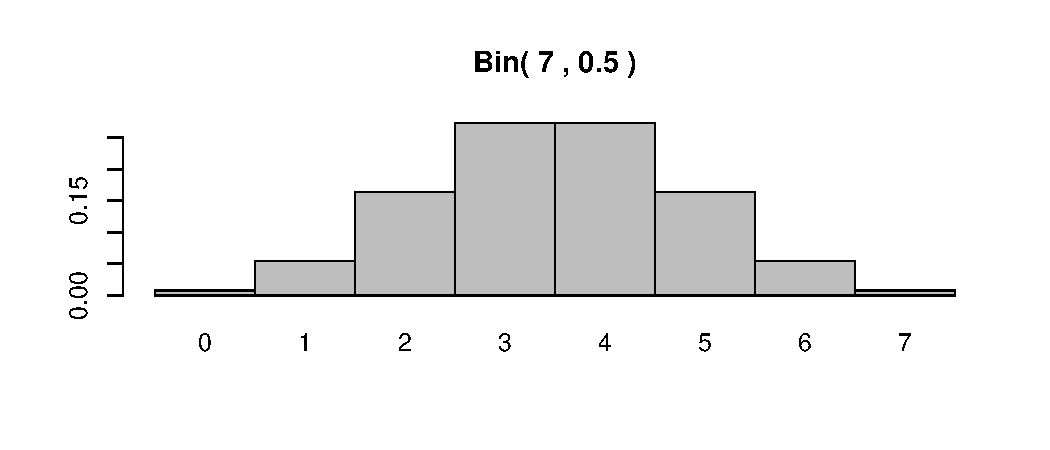
\includegraphics[width=\maxwidth]{figure/unnamed-chunk-4-1} 

\end{knitrout}
\end{frame}


\begin{frame}{}

\begin{block}{Vegetarianism}
Has vegetarianism increased in Australia?
\end{block}

\vspace{.5cm}
Let $p = P(\mbox{Vegetarian preference in Australia)}$. Note this is a 1 sided test as we are testing whether vegetarianism has `increased'.

\vspace{.5cm}
\framebox{H} 
From the 2013 data, 10\% of the Australian population choose a vegetarian diet, hence $p_{0} = 0.1$. \\
$H_{0}: p = 0.1$ vs $H_{1}: p > 0.1$. \\

\vspace{.5cm}
\framebox{A} The $n=10000$ people in the 2015 survey are independent with constant probability $p$.
\end{frame}



\begin{frame}[fragile]{}

\framebox{T} 
\begin{itemize}
\item $\tau = X =  \mbox{Number of vegetarians in the survey} \sim Bin(10000,0.1)$ under $H_{0}$. 
\item Large values of $x$ will argue against $H_{0}$ for $H_{1}$. \\
(ie if $H_{0}$ is not true, and $H_{1}$ is, then we would expect $x$ to be larger, as $p > 0.1$.).
\item The observed value is $x=1190$.
\end{itemize}

\vspace{.5cm}
\framebox{P} $P$-value = $P( X \geq 1190) \approx 0$.

\begin{knitrout}
\definecolor{shadecolor}{rgb}{0.969, 0.969, 0.969}\color{fgcolor}\begin{kframe}
\begin{alltt}
\hlnum{1}\hlopt{-}\hlkwd{pbinom}\hlstd{(}\hlnum{1189}\hlstd{,}\hlnum{10000}\hlstd{,}\hlnum{0.1}\hlstd{)}
\end{alltt}
\begin{verbatim}
## [1] 3.711557e-10
\end{verbatim}
\end{kframe}
\end{knitrout}
\end{frame}

\begin{frame}[fragile]{}

\framebox{C} 
As the $P$-value is so small, we would say that the data are not consistent with $H_{0}$. Hence, it appears that there has been an increase in vegetarianism in Australia.

\vspace{.5cm}
Note: What the $P$-value indicates, is that getting $x=1190$ or greater on a Binomial(10000,0.1) distribution is rare, which is clear from the Binomial probability distribution function.

\begin{knitrout}
\definecolor{shadecolor}{rgb}{0.969, 0.969, 0.969}\color{fgcolor}
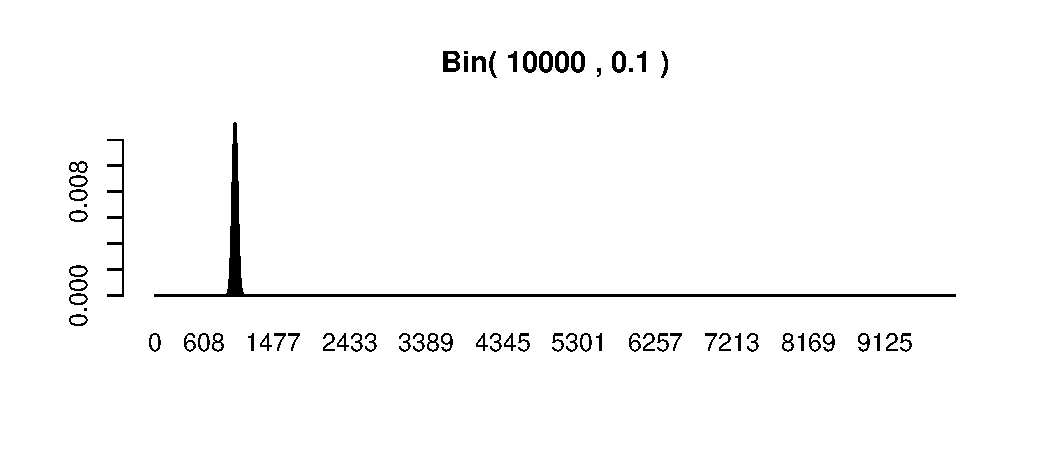
\includegraphics[width=\maxwidth]{figure/unnamed-chunk-6-1} 

\end{knitrout}
\end{frame}


\subsection[Sign Test]{Sign Test}
\begin{frame}[fragile]{Sign Test}
The Sign Test is a clever trick which effectively widens the applicability of the Proportion Test. It allows the `Proportion' Test to be used for testing for a hypothesis about a mean or median.

\vspace{.5cm}
We change from $H_{0}: \mu = \mu_{0}$ (or $H_{0}: \tilde{\mu} = \tilde{\mu}_{0}$) to $H_{0}: p_{+} = 0.5$, by considering the proportion of the signs of differences $\{ sign(x_{i}-\mu_{0})\}$ which are positive.

\vspace{.5cm}
Note:
If any observations are equal to the null hypothesis value $x_{i} = \mu_{0}$ then we eliminate them from the sample. This assumes there are only a few `zeroes', as it effectively reduces the sample size.


\end{frame}  

\begin{frame}[fragile]{}
\framebox{Context} 
\begin{itemize}
\item 
Suppose a single sample $x_{1}, x_{2}, \ldots, x_{n}$ is taken from a continuous distribution of unknown type. 
\item We want to test $H_{0}: \mu = \mu_{0}$ (or $H_{0}: \tilde{\mu} = \tilde{\mu}_{0}$).
\item
If we assume that the distribution is symmetric, then if $H_{0}$ holds, every observation is equally likely to be above or below $\mu_{0}$. 

\item Consider the set of signs of differences 
\[ sign(x_{1}-\mu_{0}), sign(x_{2}-\mu_{0}), \ldots, sign(x_{n}-\mu_{0}) \]

\item Define $X = \mbox{the number of + signs} \sim Bin(n, p_{+})$, where
$p_{+} = P(+ \mbox{ difference})$.

\item Then $H_{0}: \mu = \mu_{0}$ is equivalent to $H_{0}: p_{+} = 0.5$. 
\end{itemize}
\end{frame}  


\begin{frame}[fragile]{Steps for Sign Test}
 
\framebox{Preparation}
For $H_{0}: \mu = \mu_{0}$, calculate the signs of differences $\{ sign(x_{i}-\mu_{0}) \}$  and count the number of positive signs $x$.

\vspace{.5cm}
\framebox{H}
$H_{0}: p_{+} = 0.5$ vs $H_{1}: p_{+} < 0.5$. 

\framebox{A} The distribution is continuous and symmetric.\\
Note: For $H_{0}: \tilde{\mu} = \tilde{\mu}_{0}$, we only need to assume that the distribution is continuous. \\

\framebox{T} 
\begin{itemize}
\item $\tau = X =  \mbox{number of positive signs} \sim Bin(n,p_{+})$ (under $H_{0}$) 
\item Small values of $x$ will argue against $H_{0}$ for $H_{1}$. 
\item The observed value is $x$. 
\end{itemize}

\framebox{P} $P$-value = $P( X \leq x)$.

\framebox{C} Weigh up the size of $P$-value.

\end{frame}  


\begin{frame}{Example: Freeze Dried Coffee}

Freeze drying and spray drying are 2 different methods of producing instant coffee. The consumer is interested in the amount of caffeine residue. It is known that the median residue for freeze drying is 3.55g/100g of dry matter. This means that if $R$ is the residue (and is continuous and symmetric) that
$P(R < 3.55) = P(R > 3.55) = 0.5$. \\

In 8 samples of spray dried coffee, the residue was
\[ 4.8 , 4.0, 3.8, 4.3, 3.9, 4.6, 3.1, 3.7 \mbox{ (g/100g dry matter)} \]
{\bf Is there any difference in the caffeine residue between the 2 methods?}

\begin{center}
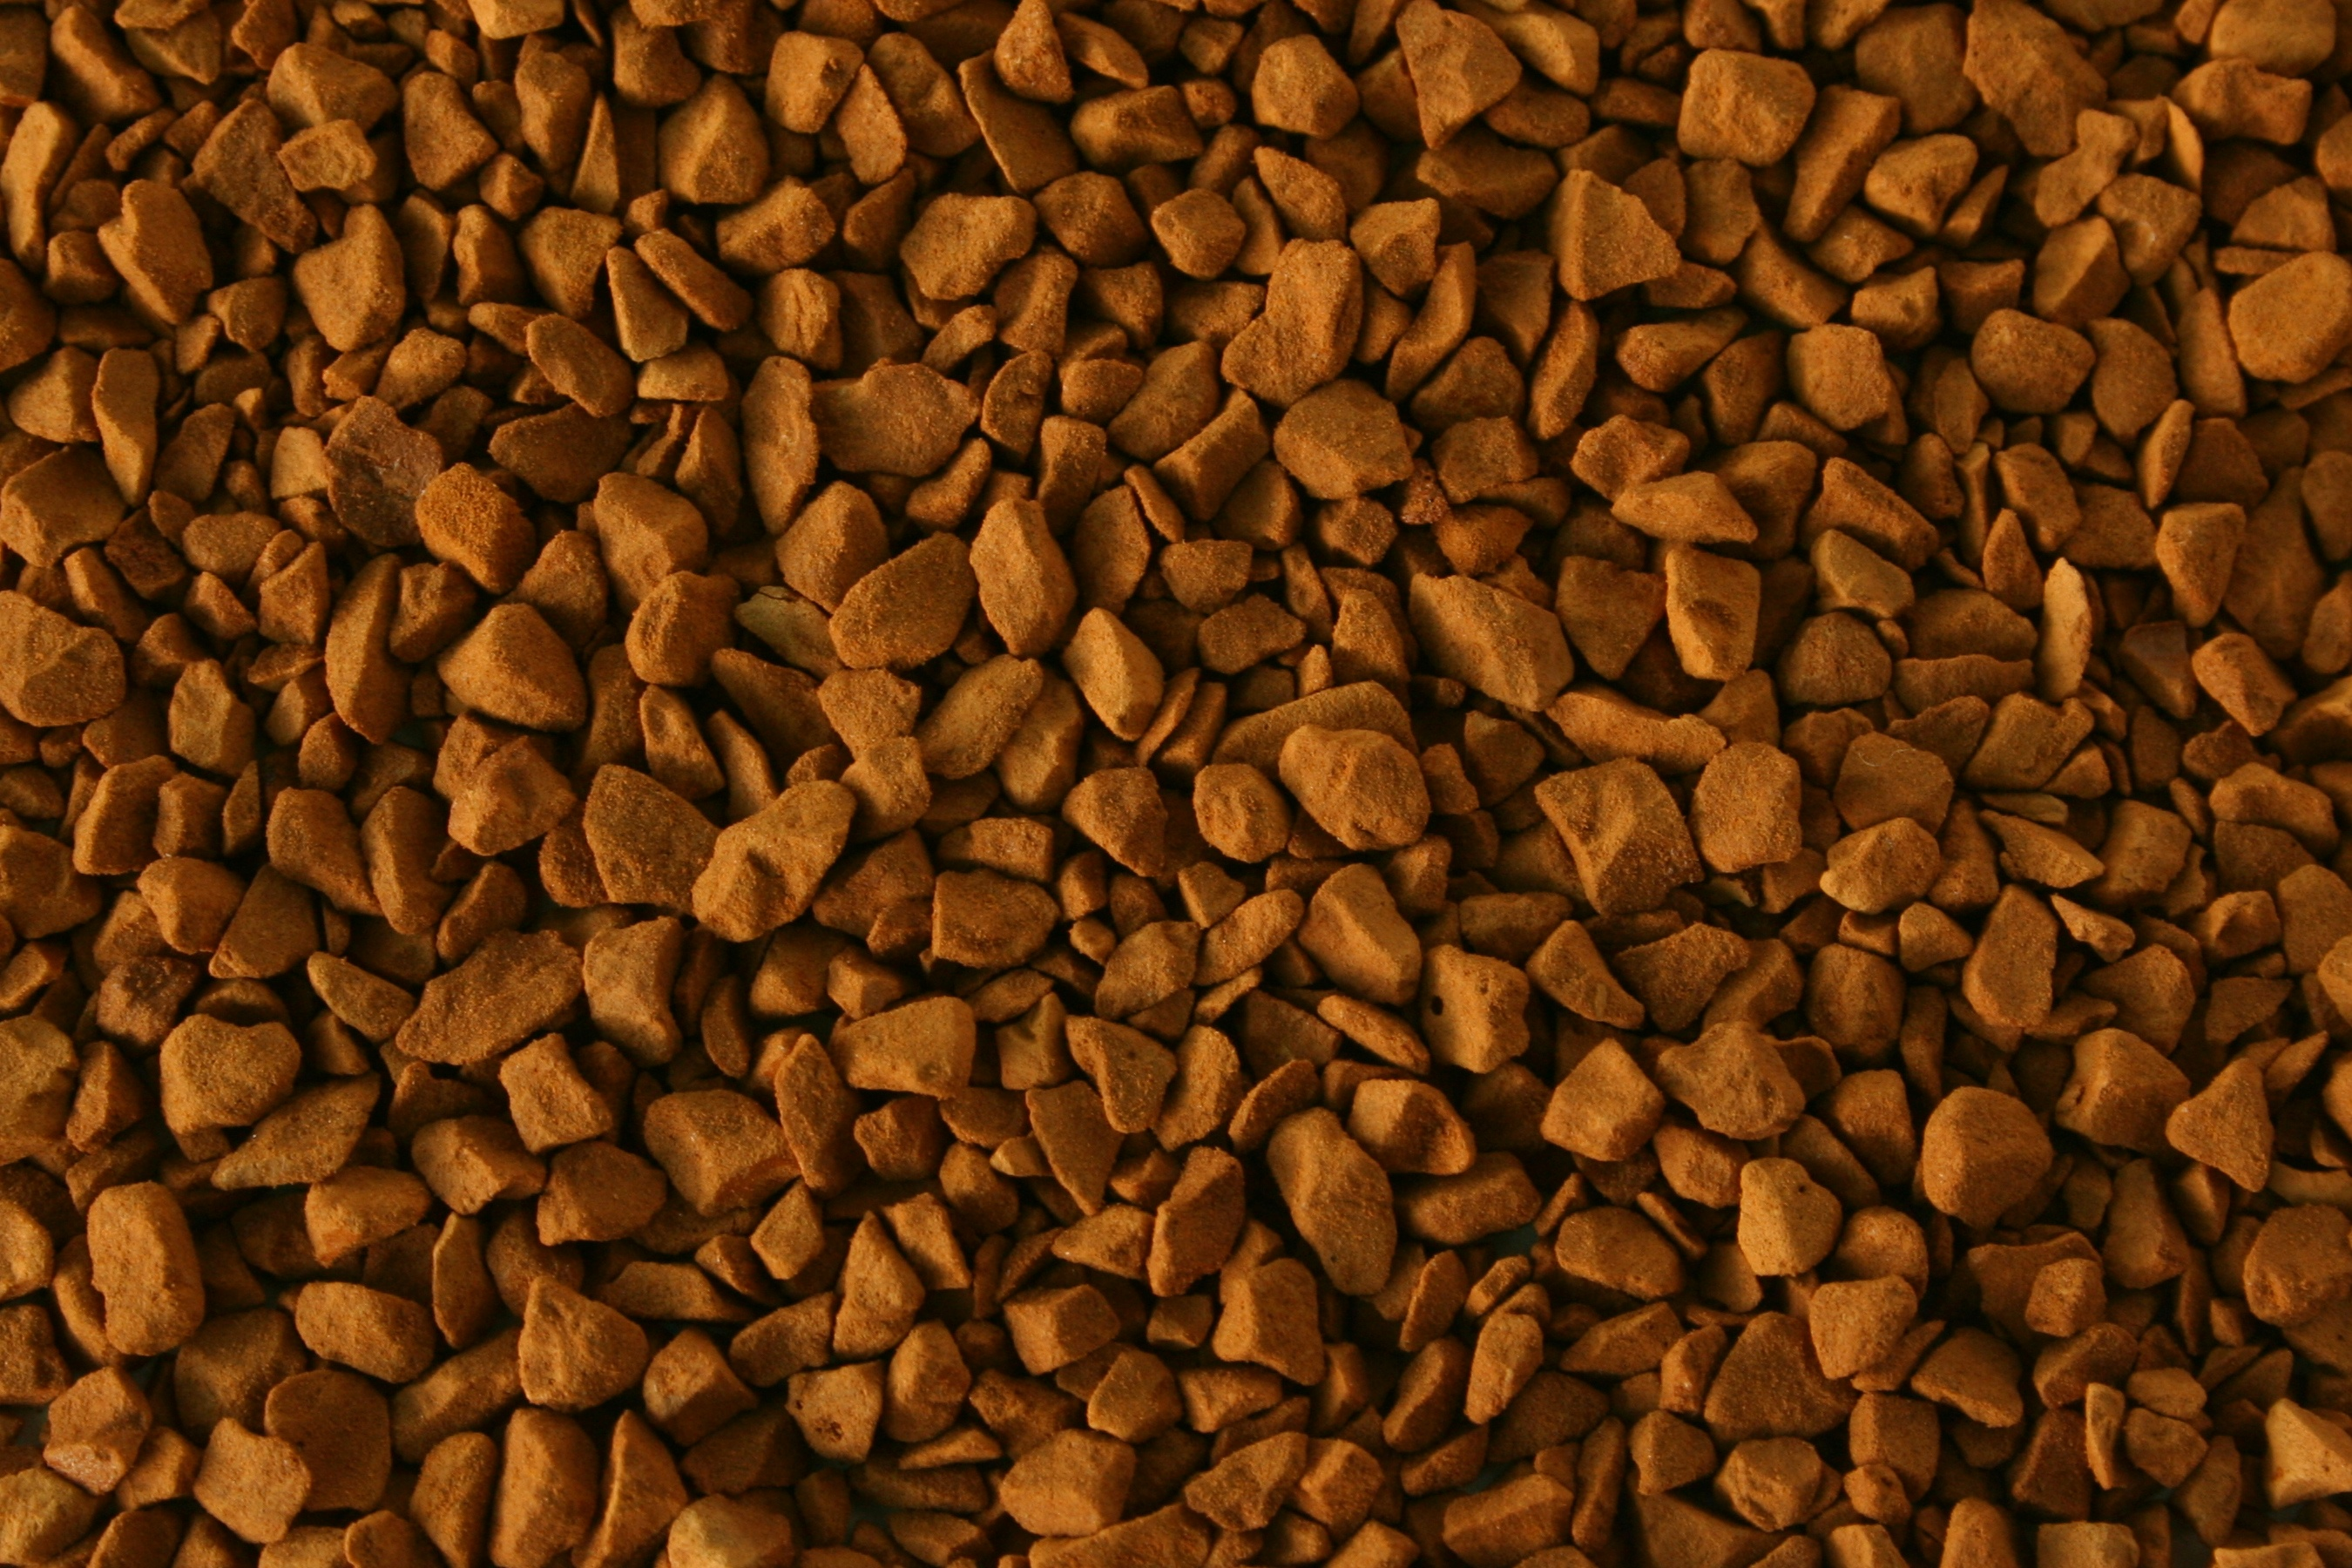
\includegraphics[height=2.5cm]{../images/FreezeCoffee.jpg}
\end{center}
\end{frame}


\begin{frame}[fragile]{}

\framebox{Preparation}
For $H_{0}: \mu = 3.55$, we calculate the signs of differences $\{ sign(x_{i}-3.55) \}$  and count the number of positive signs $x=7$.

\begin{knitrout}
\definecolor{shadecolor}{rgb}{0.969, 0.969, 0.969}\color{fgcolor}\begin{kframe}
\begin{alltt}
\hlstd{x}\hlkwb{=}\hlkwd{c}\hlstd{(}\hlnum{4.8}\hlstd{,} \hlnum{4.0}\hlstd{,} \hlnum{3.8}\hlstd{,} \hlnum{4.3}\hlstd{,} \hlnum{3.9}\hlstd{,} \hlnum{4.6}\hlstd{,} \hlnum{3.1}\hlstd{,} \hlnum{3.7}\hlstd{)}
\hlstd{x}\hlopt{-}\hlnum{3.55}
\end{alltt}
\begin{verbatim}
## [1]  1.25  0.45  0.25  0.75  0.35  1.05 -0.45  0.15
\end{verbatim}
\begin{alltt}
\hlkwd{sign}\hlstd{(x}\hlopt{-}\hlnum{3.55}\hlstd{)}
\end{alltt}
\begin{verbatim}
## [1]  1  1  1  1  1  1 -1  1
\end{verbatim}
\end{kframe}
\end{knitrout}

\vspace{.5cm}
\framebox{H}
$H_{0}: p_{+} = 0.5$ vs $H_{1}: p_{+} \neq 0.5$.  \\
This means that if the median caffeine residue is 3.55, then we should expect half the signs of differences to be positive.\\
We choose a 2 sided test, as there is no prior evidence about which method has higher caffeine residue.

\end{frame}

\begin{frame}[fragile]{}
\framebox{A} The distribution of caffeine residue is continuous and symmetric.

\vspace{.5cm}
\framebox{T} 
\begin{itemize}
\item $\tau = X =  \mbox{number of positive signs} \sim Bin(8,0.5)$ (under $H_{0}$) 
\item Large and small values of $x$ will argue against $H_{0}$ for $H_{1}$. \\
\item The observed value is $x=7$. 
\end{itemize}

\framebox{P} $P$-value = 2 $P( X \geq 7) \approx 0.07$.
(As our observed value $x=7$ is in the upper tail of the distribution, we consider $P( X \geq 7)$.

\begin{knitrout}
\definecolor{shadecolor}{rgb}{0.969, 0.969, 0.969}\color{fgcolor}\begin{kframe}
\begin{alltt}
\hlkwd{dbinom}\hlstd{(}\hlnum{7}\hlstd{,}\hlnum{8}\hlstd{,}\hlnum{0.5}\hlstd{)} \hlopt{+} \hlkwd{dbinom}\hlstd{(}\hlnum{8}\hlstd{,}\hlnum{8}\hlstd{,}\hlnum{0.5}\hlstd{)}
\end{alltt}
\begin{verbatim}
## [1] 0.03515625
\end{verbatim}
\begin{alltt}
\hlnum{1}\hlopt{-}\hlkwd{pbinom}\hlstd{(}\hlnum{6}\hlstd{,}\hlnum{8}\hlstd{,}\hlnum{0.5}\hlstd{)}
\end{alltt}
\begin{verbatim}
## [1] 0.03515625
\end{verbatim}
\end{kframe}
\end{knitrout}

\end{frame}

\begin{frame}{}

\framebox{C} As the $P$-value is 7\%, the data are consistent with $H_{0}$. \\
ie If $H_{0}$ is true, we would expect to see these data (or more extreme) 7\% of the time. It appears there is not a difference in the caffeine residue between the 2 methods of coffee production.

\vspace{1cm}
Note: To calculate the $P$-value, we can use the Binomial formula, the Binomial table, the Binomial histogram, or R.

\end{frame}




\begin{frame}{Example: Student's Sleep Study}

The Sign Test can also be applied to {\bf paired data}. Paired data is very common, for example before and after trials and studies on twins. The sign test can be used for paired data, by applying the sign test to the set of differences. \\

\vspace{.5cm}
A famous data set is Student (1908). For each of 10 patients, the amount of extra hours sleep was measured, after the administrating of 2 drugs $A$ and $B$. (A negative result indicates that the patient’s sleep reduced).  \href{https://stat.ethz.ch/R-manual/R-devel/library/datasets/html/sleep.html}{\beamergotobutton{Sleep Data}}  \\

\vspace{.5cm}
{\small \begin{tabular}{lllllllllll} \hline
Patient & 1 & 2 & 3 & 4 & 5 & 6 & 7 & 8 & 9 & 10 \\ \hline
$A$ & 0.7 & -1.6 & -0.2 & -1.2 & -0.1 & 3.4 & 3.7 & 0.8 & 0.0 & 2.0 \\
$B$ & 1.9 & 0.8 & 1.1 & 0.1 & -0.1 & 4.4 & 5.5 & 1.6 & 4.6 & 3.4 \\  \hline
\end{tabular}}
\end{frame}

\begin{frame}{}

\begin{center}
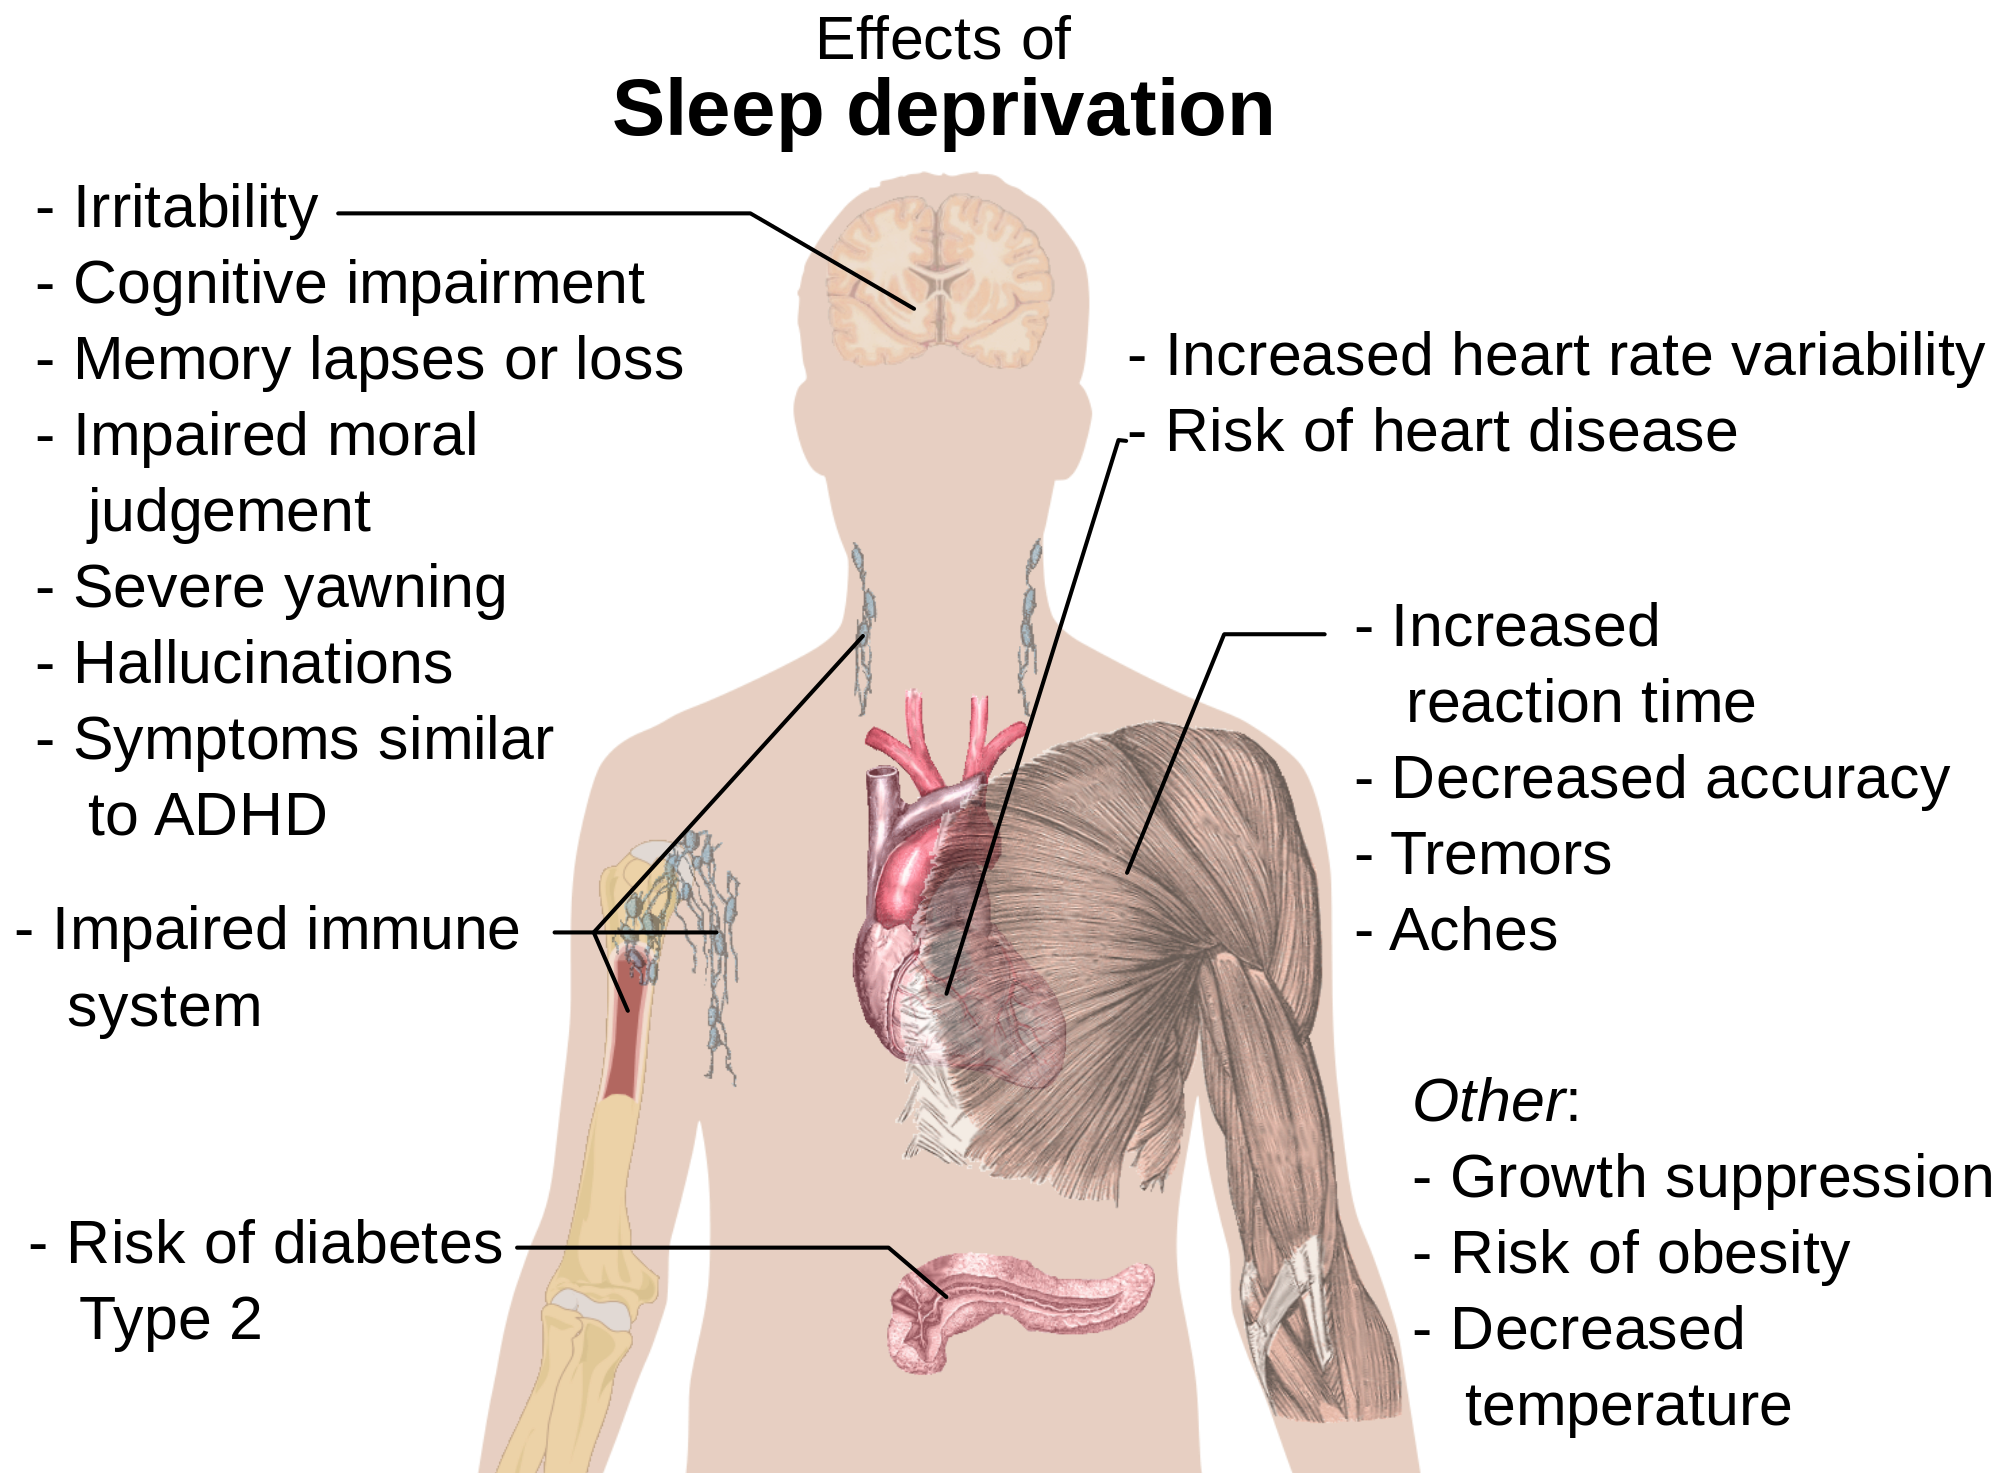
\includegraphics[height=5cm]{../images/Sleep.png}
\end{center}

{\bf Is there a difference between the affect of drugs on sleep?}

\end{frame}


\begin{frame}[fragile]{}

\framebox{Preparation}

We fill out the following table to find the differences of the paired data, and then find the signs of those differences. Notice we eliminate the 5th readings, as the difference is 0. 

\vspace{.5cm}
{\tiny \begin{tabular}{lllllllllll} \hline
Patient & 1 & 2 & 3 & 4 & 5 & 6 & 7 & 8 & 9 & 10 \\ \hline
$A$ & 0.7 & -1.6 & -0.2 & -1.2 & -0.1 & 3.4 & 3.7 & 0.8 & 0.0 & 2.0 \\
$B$ & 1.9 & 0.8 & 1.1 & 0.1 & -0.1 & 4.4 & 5.5 & 1.6 & 4.6 & 3.4 \\  \hline
$B-A$ & & & & & & & & & & \\ \hline
Sign($B-A$) & & & & & X & & & & & \\ \hline
\end{tabular}}

{\tiny 
\begin{knitrout}
\definecolor{shadecolor}{rgb}{0.969, 0.969, 0.969}\color{fgcolor}\begin{kframe}
\begin{alltt}
\hlstd{a}\hlkwb{=}\hlkwd{c}\hlstd{(}\hlnum{0.7}\hlstd{,}\hlopt{-}\hlnum{1.6}\hlstd{,}\hlopt{-}\hlnum{0.2}\hlstd{,}\hlopt{-}\hlnum{1.2}\hlstd{,}\hlopt{-}\hlnum{0.1}\hlstd{,}\hlnum{3.4}\hlstd{,}\hlnum{3.7}\hlstd{,}\hlnum{0.8}\hlstd{,}\hlnum{0.0}\hlstd{,}\hlnum{2.0}\hlstd{)}
\hlstd{b}\hlkwb{=}\hlkwd{c}\hlstd{(}\hlnum{1.9}\hlstd{,}\hlnum{0.8}\hlstd{,}\hlnum{1.1}\hlstd{,}\hlnum{0.1}\hlstd{,}\hlopt{-}\hlnum{0.1}\hlstd{,}\hlnum{4.4}\hlstd{,}\hlnum{5.5}\hlstd{,}\hlnum{1.6}\hlstd{,}\hlnum{4.6}\hlstd{,}\hlnum{3.4}\hlstd{)}
\hlstd{diff}\hlkwb{=}\hlstd{b}\hlopt{-}\hlstd{a}
\hlstd{diff}
\end{alltt}
\begin{verbatim}
##  [1] 1.2 2.4 1.3 1.3 0.0 1.0 1.8 0.8 4.6 1.4
\end{verbatim}
\begin{alltt}
\hlkwd{sign}\hlstd{(diff)}
\end{alltt}
\begin{verbatim}
##  [1] 1 1 1 1 0 1 1 1 1 1
\end{verbatim}
\end{kframe}
\end{knitrout}
}

\end{frame}

\begin{frame}[fragile]{}

For $H_{0}: \mu_{diff} = 0$, we calculate the signs of differences $\{ sign(diff_{i}-0) \}$  and count the number of positive signs $x=9$.

\vspace{.5cm}
\framebox{H}
$H_{0}: p_{+} = 0.5$ vs $H_{0}: p_{+} \neq 0.5$.  \\
This means that if the difference is 0, then we should expect half the signs of differences to be positive.\\
We choose a 2 sided test, as there is no prior evidence about which drug effects sleep more.

\vspace{.5cm}
\framebox{A} The set of differences is continuous and symmetric.

\vspace{.5cm}
\framebox{T} 
\begin{itemize}
\item $\tau = X =  \mbox{number of positive signs} \sim Bin(9,0.5)$ (under $H_{0}$) 
\item Large and small values of $x$ will argue against $H_{0}$ for $H_{1}$. \\
\item The observed value is $x=9$. 
\end{itemize}
\end{frame}

\begin{frame}[fragile]{}

\framebox{P} $P$-value = 2 $P( X \geq 9) = 2 P( X = 9) \approx 0.004$. \\
(As the observed value $x=9$ is in the upper tail of the distribution, we consider $P(X \geq 9)$.

\begin{knitrout}
\definecolor{shadecolor}{rgb}{0.969, 0.969, 0.969}\color{fgcolor}\begin{kframe}
\begin{alltt}
\hlnum{2}\hlopt{*} \hlkwd{dbinom}\hlstd{(}\hlnum{9}\hlstd{,}\hlnum{9}\hlstd{,}\hlnum{0.5}\hlstd{)}
\end{alltt}
\begin{verbatim}
## [1] 0.00390625
\end{verbatim}
\begin{alltt}
\hlnum{2}\hlopt{*} \hlstd{(}\hlnum{1}\hlopt{-}\hlkwd{pbinom}\hlstd{(}\hlnum{8}\hlstd{,}\hlnum{9}\hlstd{,}\hlnum{0.5}\hlstd{))}
\end{alltt}
\begin{verbatim}
## [1] 0.00390625
\end{verbatim}
\end{kframe}
\end{knitrout}

\begin{knitrout}
\definecolor{shadecolor}{rgb}{0.969, 0.969, 0.969}\color{fgcolor}
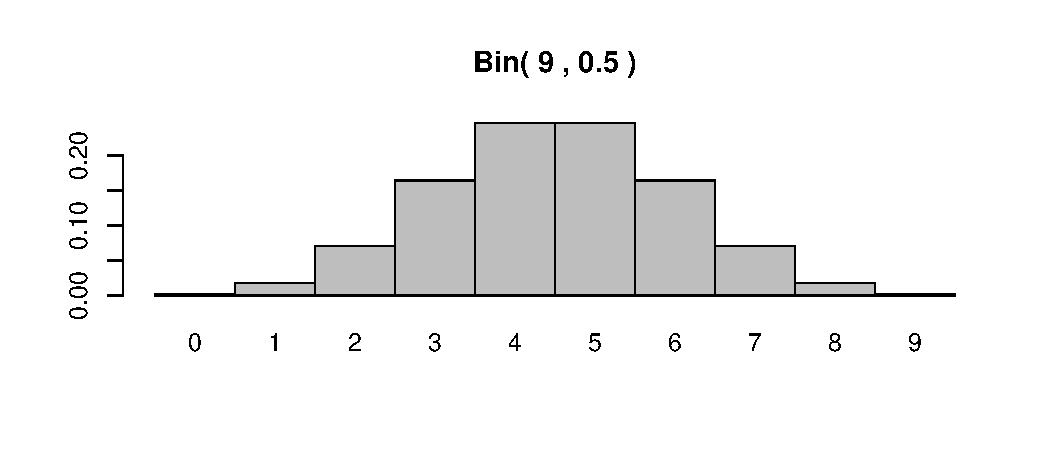
\includegraphics[width=\maxwidth]{figure/unnamed-chunk-11-1} 

\end{knitrout}
\end{frame}


\begin{frame}{}

\framebox{C} As the $P$-value is so small (0.4\%), there is strong evidence against $H_{0}$. \\
ie If $H_{0}$ is true, we would only expect to see this pattern (or more extreme) 0.4\% of the time. It appears there is a difference in the effect of the 2 drugs on sleep.
\end{frame}
\end{document}
